\problemname{Symmetric Polynomials}

\noindent
A symmetric polynomial is a polynomial in $n$ variables that remains
the same polynomial under any permutation of the variables.  For
example, $f(x_1, \ldots, x_n) = x_1 + \ldots + x_n$ is a symmetric
polynomial (it is in fact called the first elementary symmetric
polynomial).  Symmetric polynomials have many important applications.
They can, for instance, be used to prove that there is no formula for
the roots of a general five-degree polynomial.

In this problem however, we will concern ourselves with another kind
of symmetry.  Consider an infinite curve $P$ in the plane where both
$x$ and $y$ coordinates are given by polynomials, i.e.,
\begin{eqnarray*}
  x(t) & = & a_nt^n + a_{n-1}t^{n-1} + \ldots + a_1t + a_0,\\
  y(t) & = & b_mt^m + b_{m-1}t^{m-1} + \ldots + b_1t + b_0.
\end{eqnarray*}
We say that such a curve is symmetric around a straight line $L$ (given
as an equation $Ax + By + C = 0$) if there exists a real number $t_0$ such
that for all $t \in \mathbb{R}$ the point $(x(t_0+t), y(t_0+t))$ is the reflection of $(x(t_0-t),
y(t_0-t))$ around the line $L$, and we call the line $L$ a symmetry
line for the curve $P$.  For example, consider the curve $P$ given by
\begin{eqnarray*}
  x(t) & = & -5t^5 - 26t^4 - 19t^3 + 59t^2 + 111t + 26, \\
  y(t) & = & -t^5 + 17t^3 - 9t^2 - 61t + 12.
\end{eqnarray*}
This curve is symmetric around the line $5x + y + 92 = 0$ with $t_0 = -1$ (see Figure~\ref{fig:sympoly sample}).

\begin{figure}[h]
    \centering
    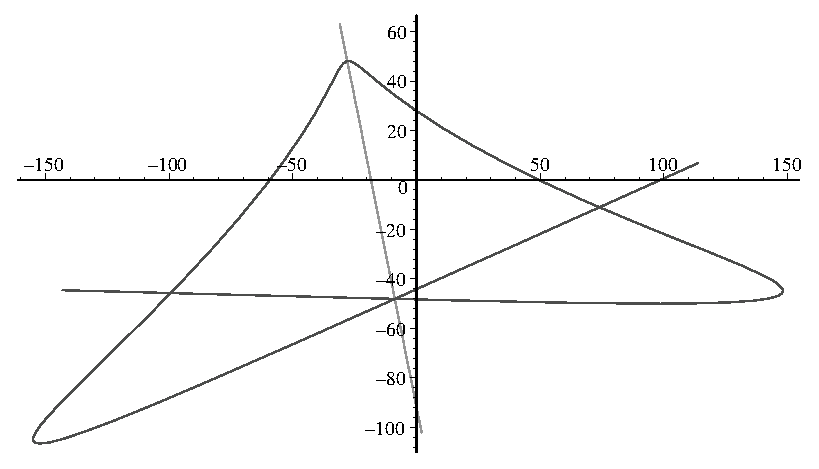
\includegraphics[width=0.6\textwidth]{poly_example}
    \caption{Illustration of Sample Input 1, drawn from $t = -3.9$ to $t = 1.9$.}
    \label{fig:sympoly sample}
\end{figure}

\noindent
Now, your task is to write a program that, given the two polynomials $x(t)$
and $y(t)$, finds a symmetry line of the curve (if one exists).

\section*{Input}

The first line of input contains an integer $n$ ($0 \le n \le 10$), the
degree of $x$.  Then follows a line with $n+1$ integers $a_n, \ldots,
a_1, a_0$, where $a_i$ is the degree $i$ coefficient of $x$.  Then
follow two lines describing the polynomial $y$ in the same format.

If either of $x(t)$ or $y(t)$ is the zero polynomial, its degree is
given as $0$.  The coefficients have absolute values bounded by
$1\,000$.  You may assume that the leading coefficient $a_n$ of each
polynomial is non-zero, except in the case when the polynomial is the
zero polynomial.

\section*{Output}

Output three real numbers $A$, $B$ and $C$, indicating that $Ax + By + C =
0$ is a symmetry line for the given curve.  If there is no symmetry
line, let $A = B = C = 0$.  If the curve has more than one symmetry line,
any one will be accepted.

In the case when a symmetry line exists, the provided line must satisfy the following conditions:
\begin{itemize}
\item $0.5 \le \max(|A|, |B|) \le 10^{100}$.
\item The direction of the provided line is within $10^{-6}$ radians of some symmetry line.
\item The value of $\frac{C}{\max(|A|, |B|)}$ is correct within an absolute or relative error of $10^{-6}$.
\end{itemize}
